\documentclass[aip,jcp,reprint,longbibliography,floatfix]{revtex4-2}

\usepackage{graphicx}
\usepackage{amsmath,amssymb,mathtools}
\usepackage{booktabs}
\usepackage{siunitx}
\usepackage{verbatim}
\usepackage{array}
\usepackage{xcolor}
\usepackage{tikz}
\usetikzlibrary{arrows.meta,backgrounds,fit,positioning}
\definecolor{FrameworkBlue}{HTML}{245C73}
\definecolor{FrameworkTeal}{HTML}{2F8F83}
\definecolor{FrameworkGold}{HTML}{C88A2D}
\definecolor{FrameworkSlate}{HTML}{4A5561}
\definecolor{FrameworkInk}{HTML}{263238}
\emergencystretch=2em

\begin{document}

\title{Algorithmic Generation and Exploitation of Topology-Aware Models for Semiexperimental Structure Refinement}

\author{Vincenzo Barone}
\email{vincebarone52@gmail.com}
\affiliation{INSTM, National Interuniversity Consortium for Materials Science and Technology, via G. Giusti 9, 50121 Firenze, Italy}

\begin{abstract}

Semiexperimental equilibrium structures combine high-resolution rotational
spectroscopy with computed vibrational and electronic corrections. The
least-squares solution of a chosen refinement model is now routine; the less
formalized step is the generation of that model. Active coordinates,
symmetry, weakly determined directions, constraints, and parameter classes are
still often selected by expert intervention, especially for cyclic, fused, and
bridged molecular graphs.

This paper introduces \texttt{MORPHEUS} (Model Optimization and Refinement from
Perceived Hierarchy, Equivalence, Uncertainty, and Symmetry), a framework that
turns model formulation into an auditable topology-perception problem. The
resulting models are not merely topology-aware: the active representation and
all constraint or parameter-class relations are topology-derived,
symmetry-consistent, rank-consistent, and recorded. Molecular topology defines
the primitive coordinate space, symmetry selects the admissible active
subspace, isotopic coverage determines which directions are supported, and
electronic-structure reference information enters only through explicit
constraints, predicates, or parameter classes.

Two equivalent active spaces are available: symmetry-adapted generalized
internal coordinates built from homogeneous primitive families, and
symmetry-adapted Cartesian displacements after removal of translations and
rotations. The chemical interface remains internal-coordinate based:
constraints, predicates, and parameter classes are expressed as primitive
bond, angle, dihedral, out-of-plane, ring, or local-frame relations and then
projected onto the selected active basis. Validation on acyclic, cyclic,
planar aromatic, fused, bridged, and flexible benchmarks shows that the same
rank, effective dimension, and rotational residuals are obtained without
manual coordinate-model formulation, while final structural parameters and
uncertainties remain chemically interpretable. A 49-atom testosterone scale
check further shows how quantum chemical equilibrium geometries, accelerated vibrational
corrections, and MORPHEUS class-constrained model generation can be
combined for large molecular systems.

\end{abstract}

\keywords{semiexperimental equilibrium structures, rotational spectroscopy, generalized internal coordinates, least squares, Kraitchman equations}

\maketitle


\section{Introduction}

Accurate equilibrium molecular structures are central to rotational
spectroscopy, thermochemistry, force-field development, and the validation of
electronic-structure methods.\cite{Demaison2011EquilibriumStructures,PuzzariniStanton2023}
Despite decades of progress in semiexperimental refinement, model construction
remains largely a manual activity. Structure determination from experimental
observables is also a
coordinate-dependent inverse problem: the data constrain a Cartesian geometry,
but the fitted variables determine conditioning, constraints, correlations, and
uncertainties. Rotational spectroscopy is a stringent example because
rotational constants probe the molecular mass distribution with high precision,
whereas semiexperimental ($r_e^{\mathrm{SE}}$) structures require vibrational
and sometimes electronic corrections to convert ground-state constants into
equilibrium information.\cite{Costain1958,Pawlowski2002,Piccardo2015B3LYP,Penocchio2015B2PLYP}

Modern fitting programs and workflows\cite{Mendolicchio2017MSR,KisielPROSPE,Kanzow2025PCCP} 
have established robust statistical principles: fit well-conditioned
observables, include theoretical predicates when experimental information is
incomplete, and propagate covariance to derived structural
parameters.\cite{Bartell1975Predicate} Their common prerequisite is that the
refinement model has already been formulated. That prerequisite is not
innocent: the active coordinates, symmetry restrictions, isotopic-coverage
assumptions, reference information, constraints, and parameter classes define
the statistical problem being solved.

This issue is modest for small acyclic molecules, but becomes central for
rings, fused systems, and bridged frameworks. A molecular graph with cycles is
not a tree; different reference paths can make one distance, angle, or torsion
primary and an equivalent one derived. For such systems, construction of a
symmetry-consistent non-redundant refinement model is itself a major part of
the semiexperimental analysis. The target of the present work is therefore
not a new least-squares observable or a molecule-specific improvement in
residuals, but an algorithmic route from perceived topology to a reproducible
statistical refinement model.

Recent automated workflows have extended semiexperimental refinement by
combining computed starting geometries, quantum chemical (QC) vibrational corrections, and
reduced-dimensionality models.\cite{Mendolicchio2025FastDvib} \texttt{MORPHEUS}
(Model Optimization and Refinement from Perceived Hierarchy, Equivalence,
Uncertainty, and Symmetry) uses such data as upstream inputs while making the
refinement model itself topology-derived. Reference geometries from QC
computations or from fragment libraries (e.g., LCB25\cite{Lazzari2025LCB25})
enter only as chemically explicit constraints, predicates, or parameter
classes; the fitted variables remain the algorithmically generated
non-redundant active coordinates. This separation is important for larger
molecules. Accurate QC equilibrium geometries and vibrational corrections are
prerequisites for a meaningful comparison with ground-state rotational
constants; the framework adds the missing step of converting those
ingredients into an explicit, rank-audited refinement model without
molecule-specific coordinate design.

The resulting topology-derived workflow starts from Cartesian coordinates. A first set
of primitive generalized internal coordinates (GICs) is built, redundancies within homogeneous
coordinate families are removed, symmetry is assigned, and the totally symmetric
active space is defined. The advisor then analyzes isotope coverage, symmetry orbits,
chemical descriptors, and reference data to generate compatible constraints,
predicates, and parameter classes. Two active spaces are available:
symmetry-adapted GICs and symmetry-adapted Cartesians obtained after removing
translations and rotations. Constraints remain primitive internal-coordinate
relations and are projected onto either active basis by the Wilson matrix or
the corresponding derivative operator.\cite{Wilson1955}

The rotational semiexperimental problem is used here as a demanding test
because it exposes both rank deficiencies and chemically meaningful
constraints. Glycolaldehyde is retained as a standard acyclic case.
Cyclopentadiene, nitrobenzene, azulene, and norcamphor test ring closures,
planar-component selection, fused topology, bridged topology, and
hydrogen-frame constraints. The maleic, phthalic, and succinic anhydrides form
a homologous literature-data series with different degrees of isotopic
completeness and different auxiliary relations. Two glycine conformers test
reduced-dimensionality constraints, and testosterone closes the study as a
large-molecule scale demonstration.


\section{Theory and Method}

\subsection{Overview of the MORPHEUS Framework}

The overall architecture is summarized in
Figure~\ref{fig:workflow-architecture}. The key separation is between the
chemical model, the numerical active basis, and the least-squares solution.
Chemical information is always expressed in primitive internal coordinates;
the active variables may be GIC amplitudes or symmetry-adapted Cartesian
displacements. This separation is what makes the generated model auditable:
the same primitive relation has the same chemical meaning regardless of the
basis used to solve the refinement.

\begin{figure*}
\centering
\resizebox{0.92\textwidth}{!}{%
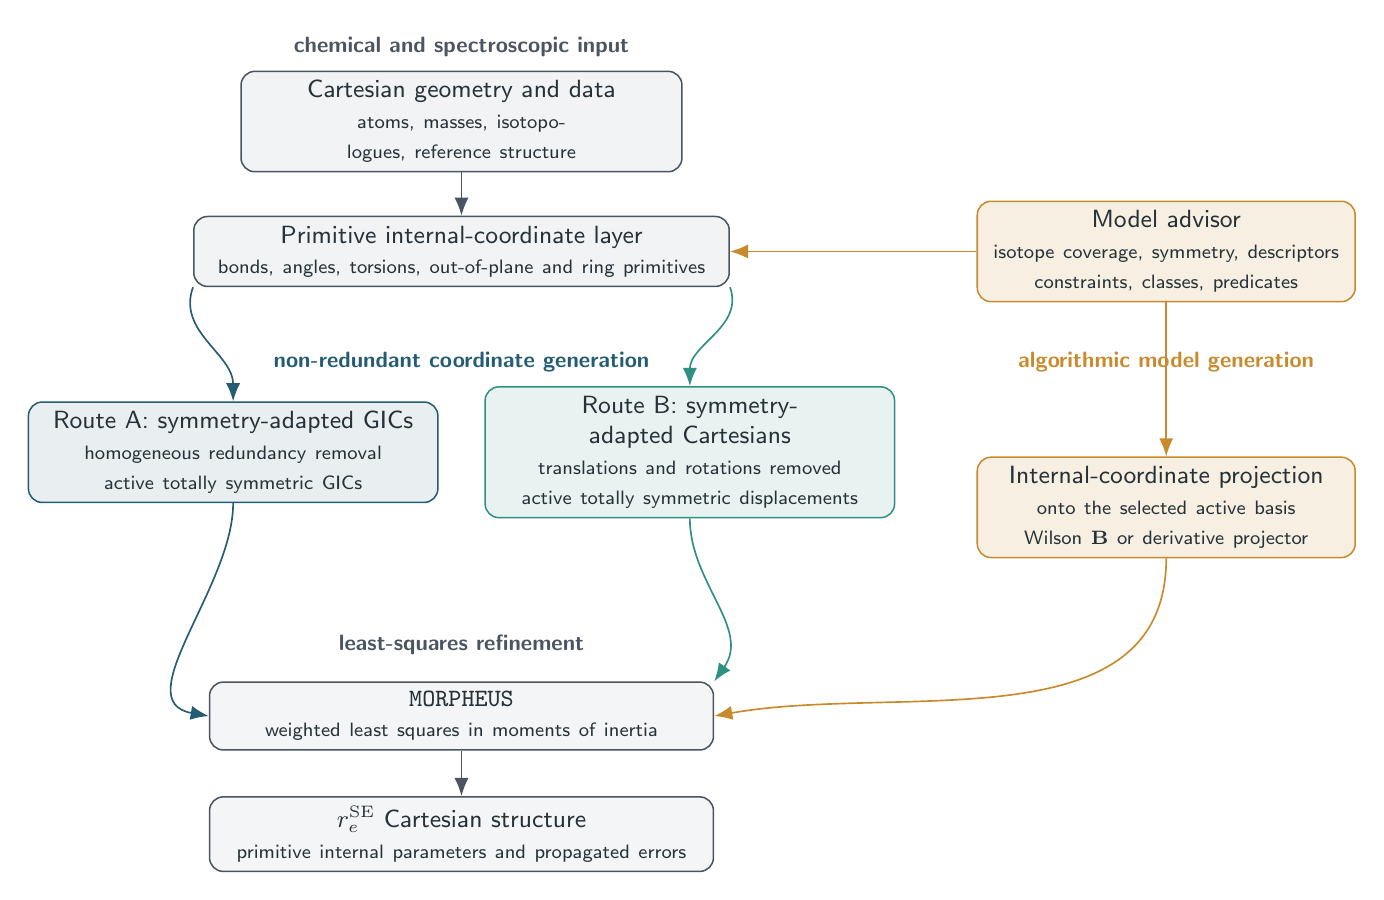
\begin{tikzpicture}[
  x=1cm,
  y=1cm,
  font=\sffamily\small,
  box/.style={
    draw,
    rounded corners=5pt,
    align=center,
    minimum height=0.82cm,
    line width=0.55pt,
    text=FrameworkInk,
    fill=white
  },
  inputbox/.style={box, fill=FrameworkSlate!7, draw=FrameworkSlate, minimum width=5.6cm, text width=5.2cm},
  primbox/.style={box, fill=FrameworkSlate!7, draw=FrameworkSlate, minimum width=6.8cm, text width=6.4cm},
  gicbox/.style={box, fill=FrameworkBlue!10, draw=FrameworkBlue, minimum width=5.2cm, text width=4.9cm},
  cartbox/.style={box, fill=FrameworkTeal!11, draw=FrameworkTeal, minimum width=5.2cm, text width=4.9cm},
  sidebox/.style={box, fill=FrameworkGold!14, draw=FrameworkGold, minimum width=4.8cm, text width=4.4cm},
  outbox/.style={box, fill=FrameworkSlate!6, draw=FrameworkSlate, minimum width=6.4cm, text width=6.0cm},
  arrow/.style={-{Latex[length=2.3mm,width=1.8mm]}, line width=0.60pt, draw=FrameworkSlate},
  gicarrow/.style={arrow, draw=FrameworkBlue},
  cartarrow/.style={arrow, draw=FrameworkTeal},
  sidearrow/.style={arrow, draw=FrameworkGold}
]
\node[font=\footnotesize\bfseries\sffamily, text=FrameworkSlate] at (-3.4,0.95) {chemical and spectroscopic input};
\node[font=\footnotesize\bfseries\sffamily, text=FrameworkBlue] at (-3.4,-3.05) {non-redundant coordinate generation};
\node[font=\footnotesize\bfseries\sffamily, text=FrameworkGold] at (5.55,-3.05) {algorithmic model generation};
\node[font=\footnotesize\bfseries\sffamily, text=FrameworkSlate] at (-3.4,-6.65) {least-squares refinement};

\node[inputbox] (geom) at (-3.4,0) {Cartesian geometry and data\\{\scriptsize atoms, masses, isotopologues, reference structure}};
\node[primbox] (prim) at (-3.4,-1.65) {Primitive internal-coordinate layer\\{\scriptsize bonds, angles, torsions, out-of-plane and ring primitives}};
\node[sidebox] (relations) at (5.55,-1.65) {Model advisor\\{\scriptsize isotope coverage, symmetry, descriptors}\\{\scriptsize constraints, classes, predicates}};

\node[gicbox] (gicroute) at (-6.3,-4.20) {Route A: symmetry-adapted GICs\\{\scriptsize homogeneous redundancy removal}\\{\scriptsize active totally symmetric GICs}};
\node[cartbox] (cartroute) at (-0.5,-4.20) {Route B: symmetry-adapted Cartesians\\{\scriptsize translations and rotations removed}\\{\scriptsize active totally symmetric displacements}};
\node[sidebox] (project) at (5.55,-4.90) {Internal-coordinate projection\\{\scriptsize onto the selected active basis}\\{\scriptsize Wilson $\mathbf{B}$ or derivative projector}};
\node[outbox] (sefit) at (-3.4,-7.55) {\texttt{MORPHEUS}\\{\scriptsize weighted least squares in moments of inertia}};
\node[outbox] (result) at (-3.4,-9.05) {$r_e^{\mathrm{SE}}$ Cartesian structure\\{\scriptsize primitive internal parameters and propagated errors}};

\draw[arrow] (geom) -- (prim);
\draw[sidearrow] (relations.west) -- (prim.east);
\draw[gicarrow] (prim.south west) to[out=-110,in=90] (gicroute.north);
\draw[cartarrow] (prim.south east) to[out=-70,in=90] (cartroute.north);
\draw[sidearrow] (relations.south) -- (project.north);
\draw[gicarrow] (gicroute.south) to[out=-90,in=170] (sefit.west);
\draw[cartarrow] (cartroute.south) to[out=-90,in=55] (sefit.north east);
\draw[sidearrow] (project.south) to[out=-90,in=10] (sefit.east);
\draw[arrow] (sefit) -- (result);
\end{tikzpicture}
}
\caption{Architecture of the \texttt{MORPHEUS} model-generation framework.}
\label{fig:workflow-architecture}
\end{figure*}


\subsection{Primitive and Work Coordinates}

The coordinate construction starts from Cartesian geometry and perceived
topology. Bonded pairs and ring connectivity define a primitive set of internal
coordinates:  stretches, valence angles, torsions, out-of-plane deformations,
linear bends, and ring-specific primitives. Redundancy is intentional at this
stage because it lets topology, not a manually chosen reference path, decide
which combinations survive. For cyclic systems, endocyclic torsions and
analogous endocyclic valence-angle combinations provide ring coordinates
within the GIC formalism, so monocyclic, fused-ring, bridged, and polycyclic
systems are handled by the same machinery.\cite{CremerPople1975} This
primitive layer is also the chemical interface for constraints, predicates,
and parameter classes.


\subsection{Coordinates for Parameter Refinement}

The active space must be non-redundant, symmetry-consistent, and compatible
with chemically meaningful constraints. In the GIC route, topological
primitives are reduced within homogeneous families, so stretches, bends,
torsions, out-of-plane motions, and ring coordinates cannot replace one
another during rank reduction.\cite{PulayFogarasi1992,Peng1996Redundant,Baker1996Delocalized,BakkenHelgaker2002}
In the Cartesian route, translations and rotations are removed from the
Cartesian displacement space. In both cases symmetry selects the totally
symmetric active block and completes primitive constraints over equivalent
orbits.

At a reference geometry $\mathbf{x}_0$, primitive displacements and Cartesian 
displacements are related to first order by the Wilson matrix\cite{Wilson1955}

\begin{equation}
\Delta \mathbf{s}
=
\mathbf{B}_s
\Delta \mathbf{x},
\qquad
\mathbf{B}_s =
\left.
\frac{\partial \mathbf{s}}
{\partial \mathbf{x}}
\right|_{\mathbf{x}_0}.
\end{equation}

For each homogeneous primitive family $\alpha$, the Wilson block

\begin{equation}
\mathbf{B}_{s_\alpha}
=
\frac{\partial\mathbf{s}_\alpha}
{\partial\mathbf{x}} .
\end{equation}

is submitted to a singular-value decomposition,\cite{GolubReinsch1970}

\begin{equation}
\mathbf{B}_{s_\alpha}
=
\mathbf{U}_{\alpha}
\boldsymbol{\Sigma}_{\alpha}
\mathbf{V}_{\alpha}^{T},
\end{equation}

The retained left-singular vectors define the row-orthonormal transformation

\begin{equation}
\mathbf{R}_{\alpha}
=
\mathbf{U}_{\alpha,r}^{T},
\end{equation}

where the subscript $r$ denotes the retained singular subspace. The
non-redundant coordinates for family $\alpha$ are then

\begin{equation}
\Delta \mathbf{q}_\alpha
=
\mathbf{R}_\alpha
\Delta \mathbf{s}_\alpha ,
\qquad
\mathbf{B}_{q_\alpha}
=
\mathbf{R}_\alpha
\mathbf{B}_{s_\alpha}.
\end{equation}

The retained rank in each family gives the number of coordinates in that
family. Stacking the blocks gives

\begin{equation}
\Delta \mathbf{q}
=
\mathbf{R}
\Delta \mathbf{s},
\qquad
\mathbf{B}_{q}
=
\mathbf{R}
\mathbf{B}_s .
\end{equation}

The block-diagonal structure preserves chemical homogeneity. A stretch can
therefore not remove a torsion from the model, and a ring coordinate cannot be
lost because a different primitive family happened to enter the rank test
first. After family-wise reduction, residual dependencies are pruned with
deterministic topological tie breaking and the final basis is checked against
the expected vibrational rank.
Cartesian displacements associated with GIC corrections use a rank-controlled
minimum-norm pseudoinverse with explicit singular-value thresholds. The
symmetry-Cartesian route uses the same selection, constraint projection, and
covariance propagation.


\subsection{Constraints, Predicates, and Parameter Classes}

Structural relations are specified in primitive internal coordinates,

\begin{equation}
\mathbf{s} = (s_1,s_2,\ldots,s_m)^T ,
\end{equation}

and may be supplied by the user or generated by the advisor. The same
projector is used for constraints, predicates, classes, and error propagation,
so changing from GICs to symmetry-adapted Cartesians changes the numerical
basis, not the primitive chemical relations that define the model.
Primitive-coordinate predicates are parsed canonically, and reversible
angle or torsion orderings are normalized before projection.

\paragraph{Hard constraints.}

Hard constraints are exact equations imposed throughout the refinement:

\begin{equation}
s_i=s_i^{0},
\end{equation}

equalities,

\begin{equation}
s_i-s_j=0,
\end{equation}

or general linearized functions,

\begin{equation}
\mathbf{c}(\mathbf{s})=\mathbf{d}.
\end{equation}

At a trial geometry the corresponding first-order condition is

\begin{equation}
\mathbf{C}_s
\Delta\mathbf{s}
=
\mathbf{b}_c,
\qquad
\mathbf{C}_s =
\left.
\frac{\partial\mathbf{c}}
{\partial\mathbf{s}}
\right|_{\mathbf{s}_0},
\qquad
\mathbf{b}_c=\mathbf{d}-\mathbf{c}(\mathbf{s}_0).
\end{equation}

Projection to the active space gives

\begin{equation}
\mathbf{C}_{A}
\Delta\mathbf{a}
=
\mathbf{b}_c,
\qquad
\mathbf{C}_{A}
=
\mathbf{C}_s
\mathbf{B}_s
\mathbf{T}_{A}.
\end{equation}

The solver keeps all compatible motions by writing the allowed correction as

\begin{equation}
\Delta\mathbf{a}
=
\Delta\mathbf{a}_0
+
\mathbf{N}\Delta\mathbf{p},
\qquad
\mathbf{C}_{A}\mathbf{N}=\mathbf{0},
\end{equation}

where $\Delta\mathbf{a}_0$ is a minimum-norm particular solution and
$\mathbf{N}$ spans the null space. The least-squares problem is solved only
for $\Delta\mathbf{p}$.

Symmetry-equivalent primitives are constrained as complete orbits before the
null-space projector is formed. Reduced-dimensionality models use the same projection, 
allowing unsupported hydrogen frames to be frozen or tied without altering the covalent topology
used for GIC generation.

\paragraph{Predicate observations.}

Predicates are soft structural information: they add weighted residuals rather
than removing degrees of freedom.\cite{Bartell1975Predicate} A primitive
predicate has the form

\begin{equation}
f(\mathbf{s})
=
f^{\mathrm{ref}}
\pm
\sigma_f ,
\end{equation}

and contributes

\begin{equation}
r_f
=
\frac{f(\mathbf{s})-f^{\mathrm{ref}}}{\sigma_f}
\end{equation}

to the residual vector. Its Jacobian with respect to the independent
least-squares variables is

\begin{equation}
\mathbf{J}_f
=
\frac{1}{\sigma_f}
\frac{\partial f}{\partial\mathbf{s}}
\mathbf{B}_s
\mathbf{T}_{A}
\mathbf{N}.
\end{equation}

\paragraph{Parameter classes.}

Parameter classes make several primitive quantities share one correction. If
class $c$ contains primitives $i\in c$, the allowed correction is

\begin{equation}
\Delta s_i
=
\Delta p_c,
\qquad
i\in c .
\end{equation}

Class definitions are converted into linear relations or Jacobian compression.
They apply to corrections rather than final values, so related quantities may
retain different reference values while sharing a fitted offset. After
convergence, the covariance is expanded back to primitive and topological
parameters.


\subsection{Semiexperimental Observables}

For each isotopologue $s$, the measured ground-state rotational constants are
converted into equilibrium rotational constants by removing vibrational and,
when necessary, electronic contributions,\cite{Costain1958,Pawlowski2002,Piccardo2015B3LYP,Penocchio2015B2PLYP}

\begin{equation}
B_{\alpha,e}^{(s)}
= B_{\alpha,0}^{(s)}
- \Delta B_{\alpha,\mathrm{vib}}^{(s)}
- \Delta B_{\alpha,\mathrm{elec}}^{(s)},
\qquad
\alpha \in \{a,b,c\}.
\end{equation}

The correction terms may come from any electronic-structure or composite
protocol and are supplied with uncertainties, masses, conventions, and
provenance.\cite{Mendolicchio2025FastDvib}

Although rotational constants may be fitted directly, the refinement uses
principal moments of inertia as default observables, because they give a smoother 
geometry dependence and avoid reciprocal amplification: 

\begin{equation}
I_{\alpha}^{(s)}
=
\frac{K}
{B_{\alpha,e}^{(s)}},
\end{equation}

where $K$ is the standard rotational conversion constant.

For planar molecules only two principal components are independent. If the
molecular plane is the $ab$ plane,

\begin{equation}
I_c = I_a + I_b ,
\end{equation}

Fitting all three components would duplicate one constraint. The workflow
therefore uses one pair, $AB$, $AC$, or $BC$, and reports the omitted component
as a diagnostic. If the pair is not specified, all admissible pairs are tested;
the selected pair maximizes rank and minimizes the propagated instability of
the omitted moment.

The selected observables and uncertainties for all isotopologues form the
experimental part of the least-squares objective.


\subsection{Least-Squares Refinement}

As usual,\cite{Demaison2011EquilibriumStructures,Mendolicchio2017MSR} the semiexperimental 
refinement is formulated as a weighted nonlinear least-squares problem. 
After hard constraints and parameter classes have been projected, the actual independent 
least-squares variables are collected in $\mathbf{p}$.

The residual vector is

\begin{equation}
\mathbf{r}
= \mathbf{y}^{\mathrm{obs}}
- \mathbf{y}^{\mathrm{calc}}(\mathbf{p}),
\end{equation}

where $\mathbf{y}$ collects all experimental observables and predicate
observations included in the refinement.

The weighted objective is

\begin{equation}
\chi^2
=
\mathbf{r}^{T}
\mathbf{W}
\mathbf{r},
\end{equation}

where $\mathbf{W}$ contains the inverse variances of experimental and predicate
observations. Robust fits reweight complete isotopologue blocks rather than
individual rotational constants, while predicates retain their assigned
statistical weights.

The optimization is performed using a weighted Levenberg--Marquardt procedure,

\begin{equation}
\left(
\mathbf{J}^{T}
\mathbf{W}
\mathbf{J}
+
\lambda \mathbf{I}
\right)
\Delta \mathbf{p}
=
\mathbf{J}^{T}
\mathbf{W}
\mathbf{r},
\label{eq:lm-step}
\end{equation}

where $\mathbf{J}$ is the Jacobian matrix of the observables with respect to
the independent variables $\mathbf{p}$ and $\lambda$ is the damping parameter.
Accepted steps are checked against the original topology, point group, 
irreducible-representation counts, and coordinate-family counts; topology-changing 
steps are rejected.

Convergence requires both parameter corrections and objective reduction to fall
below thresholds. Diagnostic leave-one-isotopologue-out refits, small singular
values, reduced rank, downweighted isotopologues, unstable planar pairs, and
large propagated coordinate uncertainties are reported without redefining the
coordinate model.

Following convergence, the covariance matrix in the independent fitted
variables is obtained from

\begin{equation}
\mathbf{C}_{p}
=
\sigma_r^2
\left(
\mathbf{J}^{T}
\mathbf{W}
\mathbf{J}
\right)^{-1},
\end{equation}

where $\sigma_r^2$ is the reduced residual variance.

\subsection{Error Propagation}

Uncertainty propagation follows the geometry-update chain. If $\mathbf{N}$ is
the null-space basis of the hard
constraints and class reductions, the covariance in the active coordinate
space is

\begin{equation}
\mathbf{C}_{a}
=
\mathbf{N}
\mathbf{C}_{p}
\mathbf{N}^{T}.
\end{equation}

The corresponding Cartesian covariance is

\begin{equation}
\mathbf{C}_{x}
=
\mathbf{T}_{A}
\mathbf{C}_{a}
\mathbf{T}_{A}^{T}.
\end{equation}

For a GIC refinement, $\mathbf{T}_{A}=\mathbf{B}_{Q}^{+}$; for a Cartesian
refinement, $\mathbf{T}_{A}=\mathbf{C}_{A_1}$. Thus both coordinate choices use
the same covariance propagation.

Reported structural quantities are functions of the optimized Cartesian
geometry. For a vector of quantities
$\mathbf{g}(\mathbf{x})$, which may contain bond lengths, valence angles,
dihedral angles, out-of-plane coordinates, ring descriptors, or user-defined
primitive functions, the covariance is

\begin{equation}
\mathbf{C}_{g}
=
\mathbf{G}_{x}
\mathbf{C}_{x}
\mathbf{G}_{x}^{T},
\qquad
\mathbf{G}_{x}
=
\left.
\frac{\partial\mathbf{g}}
{\partial\mathbf{x}}
\right|_{\mathbf{x}_{\mathrm{opt}}}.
\end{equation}

Standard errors and correlations are obtained from $\mathbf{C}_{g}$. Hard
constraints have no variance along removed directions, whereas predicate
uncertainties enter the weights and contribute to $\mathbf{C}_{p}$. 

The report lists propagated structural errors, correlations, SVD diagnostics of
the final weighted Jacobian, projected constraints and classes, and matched
active-coordinate labels. Final bond lengths, angles, dihedrals, and ring
parameters are always evaluated from the optimized Cartesian geometry, so the
reported tables are independent of whether the fit used GIC or Cartesian
amplitudes. A numerical Hessian in the final independent variable space gives
the stationary-point diagnostic.


\subsection{Kraitchman Diagnostic}

For singly substituted isotopologues, the workflow computes substitution
coordinates from the Kraitchman equations\cite{Kraitchman1953} and compares
their absolute values with the fitted coordinates in the parent principal-axis
frame. Kraitchman coordinates are widely used in spectroscopic structure work,
either directly as $r_s$ substitution coordinates, as checks on $r_0$ or
semiexperimental structures, or as practical atom-assignment diagnostics. In
this workflow they are intentionally kept outside the least-squares objective:
they are useful checks, but they do not retain coordinate signs and do not
exploit the full correlated model. At the same experimental-information level
and computational cost, the SE+fit route is therefore more informative because
all substituted constants enter one constrained Cartesian fit, uncertainties
are propagated through the same model, and the omitted planar component can
remain an external diagnostic.


\section{Implementation and Reproducibility}

The implementation is organized around two reusable services. The
coordinate-definition service builds the molecular coordinate model from
Cartesian atoms and nuclear charges, assigning point-group symmetry and
irreducible representations when requested. A separate B-matrix service
evaluates the same frozen coordinate definition for any compatible Cartesian
geometry. During refinement, the engine reuses the stored coordinate model
and updates only the derivative information needed for the current step. 

The standard input contains the Cartesian parent geometry, optional primitive
freeze or constraint records, and isotopologue data with rotational constants,
corrections, uncertainties, masses, and conventions. 

Each run records the final Cartesian structure, propagated primitive
parameters, rotational residuals, covariance and SVD diagnostics, projected
constraints/classes, provenance, warnings, and minimum-check Hessian
eigenvalues. These outputs provide the audit trail for the algorithmically
generated model and are the numerical source for the benchmark tables. 


\section{Relationship to Existing Approaches}

The framework combines established semiexperimental least-squares
machinery\cite{Mendolicchio2017MSR,Bartell1975Predicate,Mendolicchio2025FastDvib}
with an algorithmic model-generation layer. The statistical model
uses moments of inertia, vibrational and electronic corrections, predicates,
parameter classes, leverage and correlation diagnostics, robust weighting, and
final minimum checks. The new element is the formal definition and audit
trail of the refinement variables, constraints, and parameter-class structure.
Existing approaches automate the solution of a model; this work formalizes
the generation of the model itself, and then solves it with the same
statistical discipline.

Z-matrices remain compact for tree-like molecules, as illustrated below by
glycolaldehyde. Their limitations become visible for rings, fused systems, and
bridged frameworks: a molecular graph with cycles cannot be represented by a
single reference tree without making some chemically equivalent quantities
primary and others derived. In a least-squares refinement this affects not
only notation but also the covariance attached to reported parameters.

Generalized internal coordinates are a flexible alternative and are widely
used in optimization and vibrational analysis.\cite{Wilson1955,PulayFogarasi1992,Peng1996Redundant,Baker1996Delocalized,BakkenHelgaker2002,Marenich2025GIC} In those workflows the generalized coordinates are usually a user-defined
layer. Here they are generated from topology-based primitive coordinates,
reduced to a non-redundant space, assigned to irreducible representations, and
accessed through primitive-coordinate constraints. Kisiel's
\texttt{STRFIT}/PROSPE route\cite{KisielPROSPE} provides another important
reference point for rotational-structure fitting, but the structural model is
again supplied by the user and may leave derived ring quantities outside the
primary fitted covariance matrix.\cite{Kanzow2025PCCP}

The practical distinction is summarized in Table~\ref{tab:workflow-comparison}.
The workflow retains the usual semiexperimental inputs and diagnostics while
moving coordinate construction, symmetry completion, constraint and class
generation, and covariance propagation to a common topology-derived layer. The
user still controls the chemical problem and the quality of the input data;
what is removed is the need to hand-build the non-redundant refinement model.

\begin{table*}
\caption{Compact operational comparison of representative
structure-refinement routes. The emphasis is model formulation rather than the
statistical quality of a particular fit.}
\label{tab:workflow-comparison}
\scriptsize
\setlength{\tabcolsep}{4pt}
\begin{tabular}{@{}llll@{}}
\toprule
Feature & Z-matrix & User GIC or PROSPE & \texttt{MORPHEUS} \\
\midrule
Input model & Internal tree & User model & Cartesian topology \\
Active variables & Manual & Manual & Auto rank-pruned \\
Rings/bridges & Tree-dependent & User-defined & Auto primitives \\
Missing isotopes & Manual constraints & Manual classes & Advisor constraints \\
Symmetry & In model & User supplied & Detected and audited \\
Output audit & Supplied model & Workflow dependent & Manifest and covariance \\
\bottomrule
\end{tabular}
\end{table*}


\subsection{Computational Reference Data}

The electronic-structure quantities used in this work were generated with the
hierarchical family of Pisa composite schemes (PCSs). In most cases,
vibrational corrections and constraint targets were taken from the
double-hybrid member of the family (DPCS3), which has been validated in
previous work for accurate structures and fast rovibrational corrections. The
only exception is conformer I of glycine, where the best available reference
was used: PCS4, based on explicitly correlated CCSD(T)-F12 calculations close
to the complete-basis-set limit with an additive core--valence correction.
Outside this role as reference information, the electronic-structure data do
not define the fitted coordinates; they enter only through explicit
constraints, predicates, parameter classes, and $\Delta B_\mathrm{vib}$
corrections.


\section{Results and Discussion}

The systems are discussed in the order in which they test increasingly
demanding parts of the same algorithmic model-generation problem. Glycolaldehyde is
the acyclic reference case; cyclopentadiene tests ring closure; nitrobenzene
and azulene test planar-component selection and fused aromatic topology;
norcamphor tests bridged graphs and hydrogen-frame constraints. The anhydride
series then probes how published data sets with different isotopic
completeness are converted into equivalent input models. Glycine I and II test
reduced-dimensionality constraints. Testosterone is kept separate and last
because it is a scale demonstration rather than an isotope-rich benchmark. In
all cases the input is Cartesian and no molecule-specific coordinate code,
manual reference tree, or manual active-space selection is used.

\begin{figure*}
\centering
\begin{minipage}{0.23\linewidth}
\centering
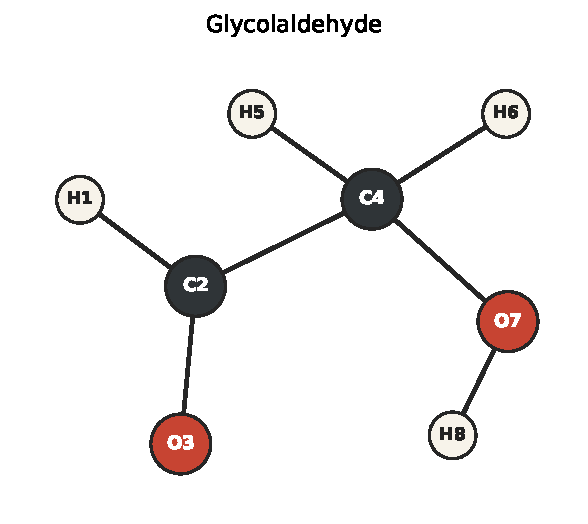
\includegraphics[width=\linewidth]{figures/glycolaldehyde_numbering.pdf}
\end{minipage}
\begin{minipage}{0.23\linewidth}
\centering
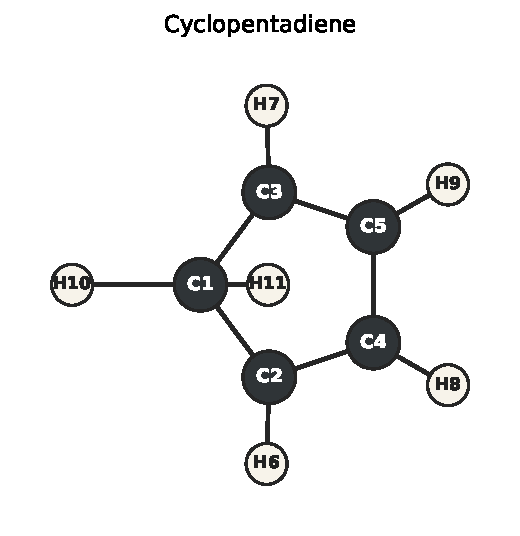
\includegraphics[width=\linewidth]{figures/cyclopentadiene_numbering.pdf}
\end{minipage}
\begin{minipage}{0.23\linewidth}
\centering
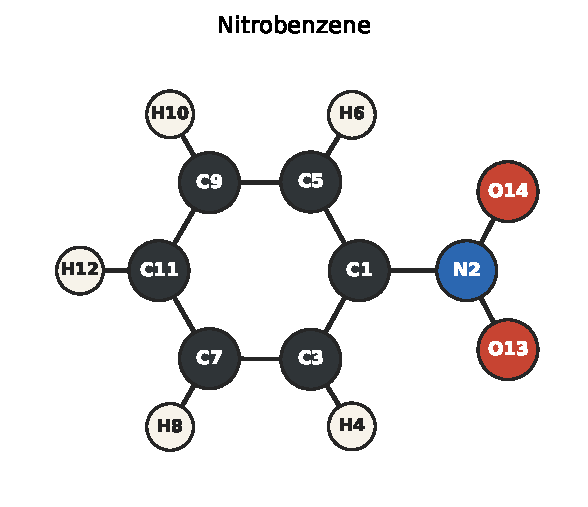
\includegraphics[width=\linewidth]{figures/nitrobenzene_numbering.pdf}
\end{minipage}
\begin{minipage}{0.23\linewidth}
\centering
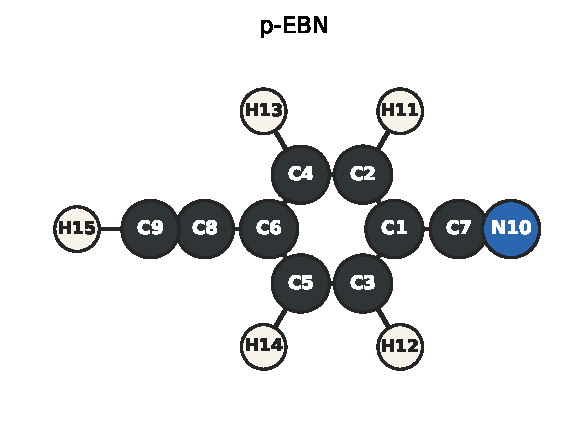
\includegraphics[width=\linewidth]{figures/p-EBN_numbering.pdf}
\end{minipage}

\vspace{0.25em}

\begin{minipage}{0.23\linewidth}
\centering
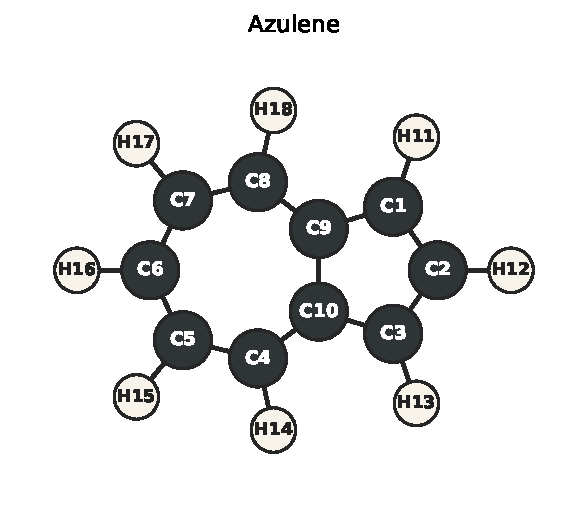
\includegraphics[width=\linewidth]{figures/azulene_numbering.pdf}
\end{minipage}
\begin{minipage}{0.23\linewidth}
\centering
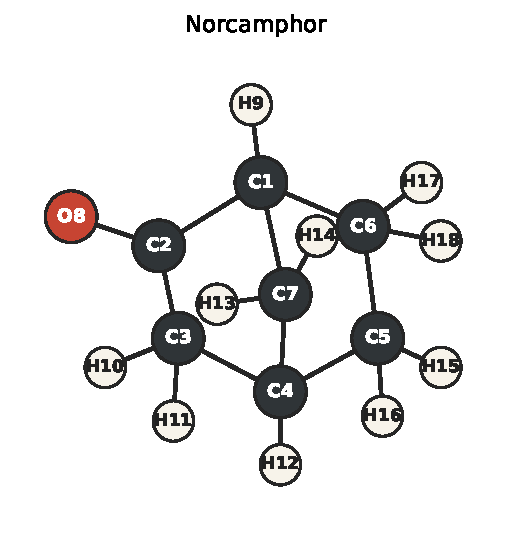
\includegraphics[width=\linewidth]{figures/norcamphor_numbering.pdf}
\end{minipage}
\begin{minipage}{0.23\linewidth}
\centering
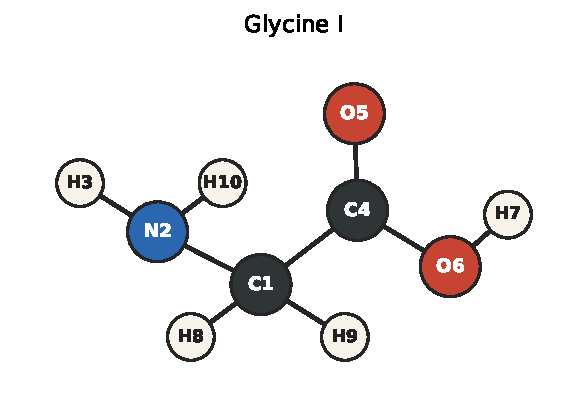
\includegraphics[width=\linewidth]{figures/glycine_I_numbering.pdf}
\end{minipage}
\begin{minipage}{0.23\linewidth}
\centering
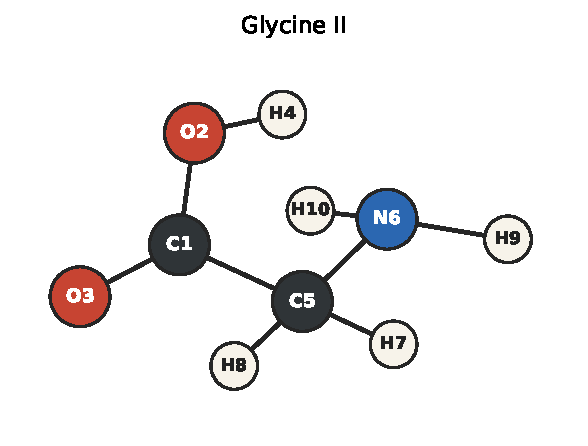
\includegraphics[width=\linewidth]{figures/glycine_II_numbering.pdf}
\end{minipage}

\vspace{0.25em}

\begin{minipage}{0.23\linewidth}
\centering
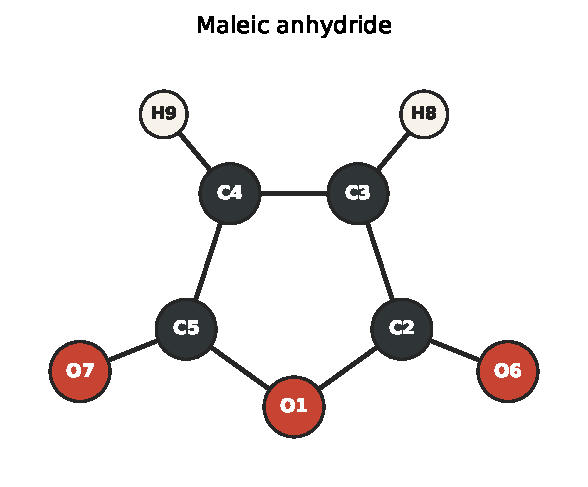
\includegraphics[width=\linewidth]{figures/maleic_anhydride_numbering.pdf}
\end{minipage}
\begin{minipage}{0.23\linewidth}
\centering
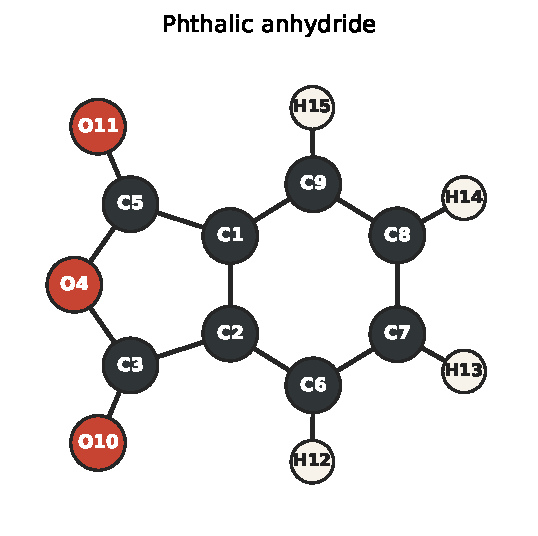
\includegraphics[width=\linewidth]{figures/phthalic_anhydride_numbering.pdf}
\end{minipage}
\begin{minipage}{0.23\linewidth}
\centering
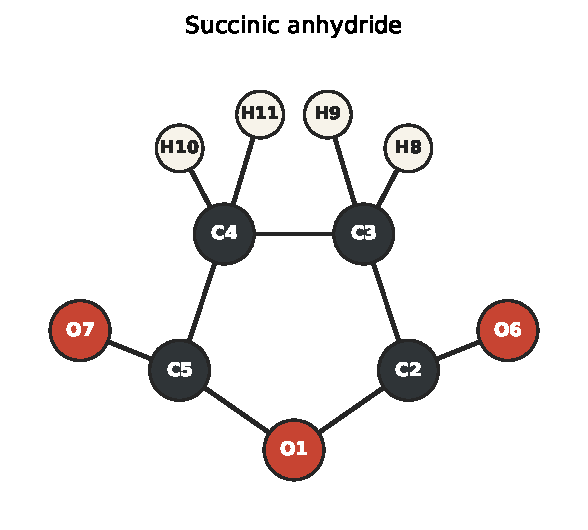
\includegraphics[width=\linewidth]{figures/succinic_anhydride_numbering.pdf}
\end{minipage}
\caption{Structures and atom numbering for the validation systems used to test algorithmic
model generation: glycolaldehyde, cyclopentadiene, nitrobenzene, p-EBN,
azulene, norcamphor, glycine I, glycine II, and the maleic, phthalic, and
succinic anhydride series. For these systems, the same Cartesian
numbering is used by topology perception, coordinate generation, constraints,
diagnostics, and final structural tables.}
\label{fig:studied-structures}
\end{figure*}

\begin{figure*}
\centering
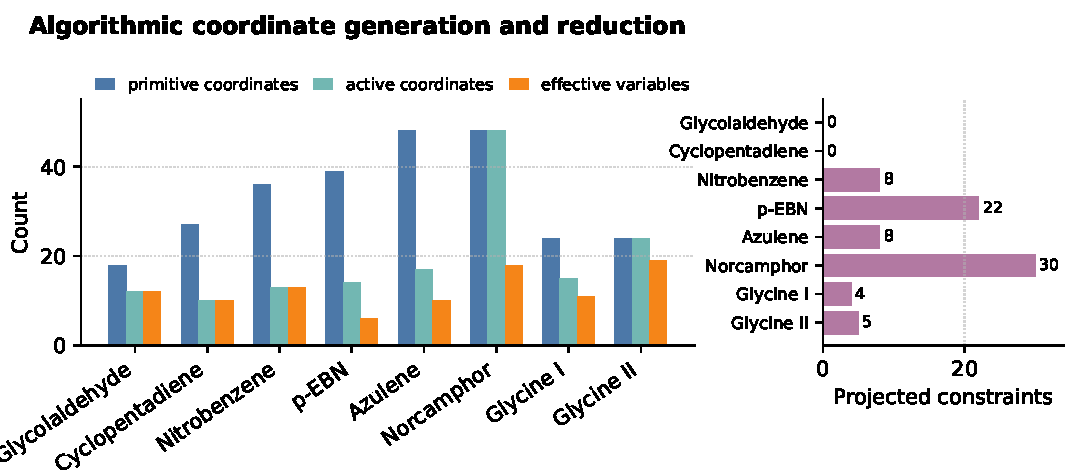
\includegraphics[width=0.92\linewidth]{figures/benchmark_overview.pdf}
\caption{Algorithmic model-generation audit for the representative
refinements. The left panel reports the number of coordinates generated
algorithmically, the symmetry-active subset before constraint
projection, and the final least-squares variables after reduction. The right
panel reports the number of constraints or frozen primitive parameters
projected by the model layer. Manual coordinate-model edits are zero for every
case. Detailed fit residuals and ranks are collected in the Supporting
Information.}
\label{fig:benchmark-overview}
\end{figure*}

Figure~\ref{fig:benchmark-overview} is the central validation of the framework:
it quantifies how topology perception, symmetry analysis,
isotopic coverage, and reference information are transformed algorithmically
into the final refinement model. The figure is therefore a
model-generation audit, not simply a residual summary: it reports how many
primitive/non-redundant coordinates are produced by the algorithmic generator, how many
remain active after symmetry selection, how many survive constraint
projection, and how many constraints are introduced without manual parameter
selection. The rotational residuals remain in the expected semiexperimental
range for standard, cyclic, planar, fused, bridged, and glycine benchmarks,
but the central result is that these residuals are obtained from generated,
auditable models. The glycine examples also separate two roles of theory:
Gly-I starts from a reference that already satisfies the practical
rotational-accuracy target, whereas Gly-II uses QC-derived relations to define
missing reduced-dimensionality information.

Figure~\ref{fig:benchmark-overview} also makes explicit what is generated.
For azulene, topology and symmetry generate 48 final GICs, identify 17
totally symmetric coordinates, and reduce the fit to 10 effective variables
without a manual choice of refined coordinates. For norcamphor, the same
machinery constructs a non-redundant 48-coordinate GIC model for a
low-symmetry bridged system, then generates 30 hydrogen-frame constraints and
leaves 18 effective variables. These are the cases in which manual model
formulation is most exposed: fused rings and bridged frameworks make it
difficult to decide by inspection which distances, angles, torsions, and
hydrogen-frame quantities should be refined, tied, or constrained.
Table~\ref{tab:manual-vs-morpheus} recasts the same information as model-
formulation burden. The manual column lists the decision classes that would
normally have to be settled before the least-squares fit; the generated column
reports the resulting working model and residuals. Stretches, bends, torsions,
out-of-plane terms, linear bends, and ring-deformation coordinates are generated
from the perceived graph and reduced in homogeneous families. Consequently, a
stretching coordinate cannot replace a torsion or a ring coordinate during rank
reduction.

\begin{table*}
\caption{Decision burden removed by algorithmic model generation. Manual setup time
is not reported because it depends on operator choices; the table therefore
reports the reproducible decision burden. The final column counts
molecule-specific coordinate or constraint edits made by the user in the
reported runs.}
\label{tab:manual-vs-morpheus}
\scriptsize
\setlength{\tabcolsep}{3.5pt}
\resizebox{\textwidth}{!}{%
\begin{tabular}{@{}llllll@{}}
\toprule
Case & Manual workflow would decide & Generated model & Constraints/classes & Result & Manual edits \\
\midrule
Azulene &
fused-ring coordinates; symmetry; active variables; planar pair &
48 GICs; 17 symmetric; 10 variables &
8 primitive constraints &
0.073 MHz RMS &
0 \\
Norcamphor &
bridged coordinates; active variables; H-frame constraints; covariance targets &
48 GICs; 48 active; 18 variables &
30 H-frame constraints &
0.071 MHz RMS &
0 \\
Glycine I &
symmetry; unsupported H-frame directions; active variables &
24 GICs; 15 $A'$; 11 variables &
4 QC constraints &
0.0269 MHz RMS &
0 \\
Glycine II &
low-symmetry active space; coupled descriptors; unsupported directions &
24 GICs; 19 variables &
5 QC constraints; coupled classes &
0.249 MHz RMS &
0 \\
\bottomrule
\end{tabular}
}
\end{table*}

The agreement with reference-quality refinements is therefore obtained after
removing the molecule-specific model-design step, not after tuning it.

The three anhydrides were selected as a homologous literature-data series, not
as unrelated examples. They have the same chemical motif but progressively
different experimental completeness, and therefore test different parts of
the workflow. Maleic anhydride is the fully determined case: the published
work of Vogt, Demaison, and Rudolph\cite{Vogt2011MaleicAnhydride} reports the
parent geometry, ground-state rotational constants, rovibrational corrections,
and semiexperimental constants for a sufficiently rich isotopic set. Phthalic
anhydride tests mixed estimation: Belyakov et
al.\cite{Belyakov2022PhthalicAnhydride} supplement the rotational data with
weighted $r_e^\mathrm{BO}$ predicates. Succinic anhydride tests the opposite
limit: Jahn et al.\cite{Jahn2020SuccinicAnhydride} provide only heavy-atom
substitutions, so the hydrogen frame is not experimentally resolved and must be
represented by explicit model relations.

This series also makes the input claim concrete. Once $B_0$ constants and
rovibrational corrections $\Delta B_\mathrm{vib}$ are available, the
user transcribes the parent Cartesian geometry, the isotope
substitutions, and the tabulated corrections. The program then perceives the
topology and symmetry, constructs the non-redundant coordinate model, and
the model layer applies any necessary constraints, predicates, or parameter
classes as explicit statistical relations.

For maleic anhydride no auxiliary relation is introduced and 21
non-redundant symmetry coordinates are generated, of which the eight $A_1$ coordinates are
the active variables for the planar SE fit (Table~\ref{tab:maleic-symmetry-gics}).
The GIC and symmetry-Cartesian routes both give rank 8 and a rotational RMS
residual of 0.036~MHz; the recovered bond lengths agree with the published
$r_e^\mathrm{SE}$ values within $1.2\times10^{-4}$~\AA.

\begin{table*}[t]
\caption{Algorithmically generated symmetry-coordinate model for maleic
anhydride from literature data. Only the totally symmetric $A_1$ block is
active in the C$_{2v}$ semiexperimental refinement.}
\label{tab:maleic-symmetry-gics}
\scriptsize
\setlength{\tabcolsep}{4pt}
\begin{tabular}{@{}lcl@{}}
\toprule
Symmetry block & Coordinates & Role in the SE model \\
\midrule
$A_1$ & 8 & Active stretches/bends; rank 8 \\
$A_2$ & 3 & Torsion/out-of-plane diagnostics \\
$B_1$ & 3 & Torsion/out-of-plane diagnostics \\
$B_2$ & 7 & Stretch/bend diagnostics \\
\midrule
Total & 21 & Non-redundant GIC space \\
\bottomrule
\end{tabular}
\end{table*}

Table~\ref{tab:generated-relation-example} illustrates the type of chemically
meaningful relations generated by the advisor. The user does
not select active coordinates or construct a Z-matrix; instead, the program
identifies unsupported structural directions and expresses them as primitive
internal-coordinate relations, which are subsequently projected onto the
algorithmically generated active space. The same representation also makes
ring coordinates explicit: endocyclic bends and torsions are generated as
linear combinations of primitive valence angles or dihedral angles rather than
as molecule-specific coordinate choices.

\begin{table*}[t]
\caption{Chemically readable primitive-coordinate relations generated by the
model layer. The first four entries are representative reduced-dimensionality
constraints for glycine; the last two show the corresponding form of generated
ring coordinates. Atom labels are used for readability.}
\label{tab:generated-relation-example}
\scriptsize
\setlength{\tabcolsep}{4pt}
\begin{tabular}{@{}lll@{}}
\toprule
Primitive relation & Generated relation & Role \\
\midrule
O--H bond & \texttt{ROH = R(O,H)} & fixes unsupported O--H distance \\
C--O--H angle & \texttt{AOH = A(C,O,H)} & preserves hydroxyl orientation \\
H--N--H angle & \texttt{HNH = A(H,N,H')} & constrains amino frame \\
NH$_2$ wag & \texttt{WNH2 = OOP(H,N,H',C)} & removes unsupported wagging direction \\
Endocyclic bend & \texttt{RB = sum c(i) A(i,j,k)} & defines ring valence coordinate \\
Endocyclic torsion & \texttt{RT = sum c(i) D(i,j,k,l)} & defines ring puckering/torsional coordinate \\
\bottomrule
\end{tabular}
\end{table*}

For phthalic anhydride, the rotational information alone can give a small
rotational residual while leaving the structural model rank deficient. The
published solution is therefore naturally expressed as primitive-coordinate
predicates with conservative uncertainties of 0.002~\AA{} for bond lengths and
0.2$^\circ$ for angles. With these predicates, the fit has
rank 14, condition number 4.05, and a rotational RMS residual of 0.50~MHz. It
recovers the published $r_e^\mathrm{SE}$ structure within 0.0015~\AA{} for the
tabulated bond lengths and within 0.09$^\circ$ for the tabulated angles.

\begin{table*}[t]
\caption{Effect of auxiliary model relations for phthalic anhydride. The
predicate model uses the conservative $r_e^\mathrm{BO}$ uncertainties reported
by Belyakov et al. and the same literature rotational data. Structural errors are 
maximum absolute deviations from the tabulated $r_e^\mathrm{SE}$ bond lengths or angles.}
\label{tab:phthalic-predicates}
\scriptsize
\setlength{\tabcolsep}{2.5pt}
\begin{tabular}{lcccc}
\toprule
Auxiliary relation & Rank & Cond. & RMS & Error \\
\midrule
None & 13 & $\infty$ & 0.0065 & 3.13$^\circ$ \\
Frozen H frames & 9 & 1056 & 0.0067 & 0.19$^\circ$ \\
$r_e^\mathrm{BO}$ predicates & 14 & 4.05 & 0.50 & 0.0015~\AA; 0.09$^\circ$ \\
\bottomrule
\end{tabular}
\end{table*}

Succinic anhydride completes the series because only heavy atoms are
isotopically substituted. The heavy-atom framework is determined, but the
hydrogen positions are not independent spectroscopic observables. In this case
a local hydrogen-frame constraint gives a stable fit with rank 5 and a
rotational RMS residual of 0.035~MHz. Weighted C--H predicates are still useful
diagnostically, but as soft observations they do not remove all unobserved
hydrogen-frame directions; without an additional topological or constraint
relation the optimizer can enter geometrically equivalent but chemically
unacceptable valleys. The comparison makes the distinction operational:
constraints remove unsupported directions, predicates add observations with
declared uncertainty, and parameter classes tie equivalent corrections. 

\begin{figure}
\centering
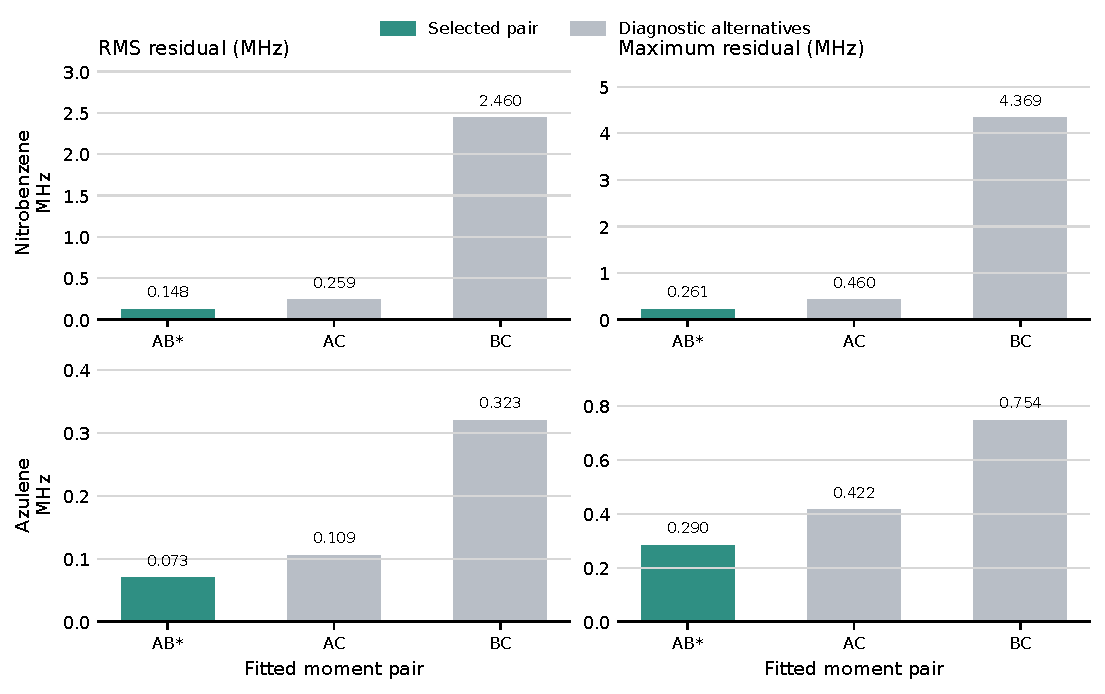
\includegraphics[width=0.82\linewidth]{figures/planar_pair_diagnostics.pdf}
\caption{Planar-component selection for nitrobenzene and azulene: the selected 
$AB$ pair is highlighted and minimizes the complete post-fit diagnostic residual 
while the omitted component remains
an external check. Detailed values are reported in the Supporting Information.}
\label{fig:planar-pair-diagnostics}
\end{figure}

For planar molecules the model layer selects the best pair of rotational
constants to be fitted, and retains the third rotational constant as
an external check computed from the final Cartesian geometry.
Figure~\ref{fig:planar-pair-diagnostics} shows that the $AB$ pair gives the
smallest complete diagnostic residual for both nitrobenzene and azulene.

\begin{figure}
\centering
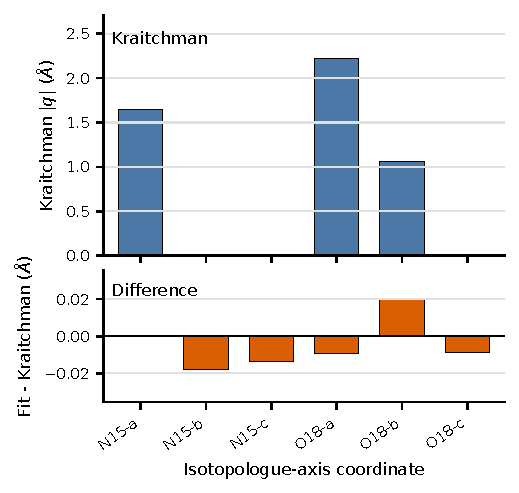
\includegraphics[width=0.92\linewidth]{figures/nitrobenzene_kraitchman_fit.pdf}
\caption{Kraitchman diagnostic for the nitrobenzene planar benchmark. The
upper panel reports absolute substitution coordinates from the Kraitchman
analysis. The lower panel reports signed differences between the final SE
coordinates and the Kraitchman values on an expanded scale. Numerical values
are reported in the Supporting Information.}
\label{fig:nitrobenzene-kraitchman-fit}
\end{figure}

The next two diagnostics compare the fitted structures with independent
structural information without changing the least-squares objective. The
nitrobenzene Kraitchman comparison in
Figure~\ref{fig:nitrobenzene-kraitchman-fit} confirms that the fitted
Cartesian structure follows the substitution-coordinate pattern, while the fit
itself remains based on moments of inertia. This is the intended use of
Kraitchman information here: it validates the SE+fit geometry but does not
replace the statistically coupled refinement.

\begin{figure*}
\centering
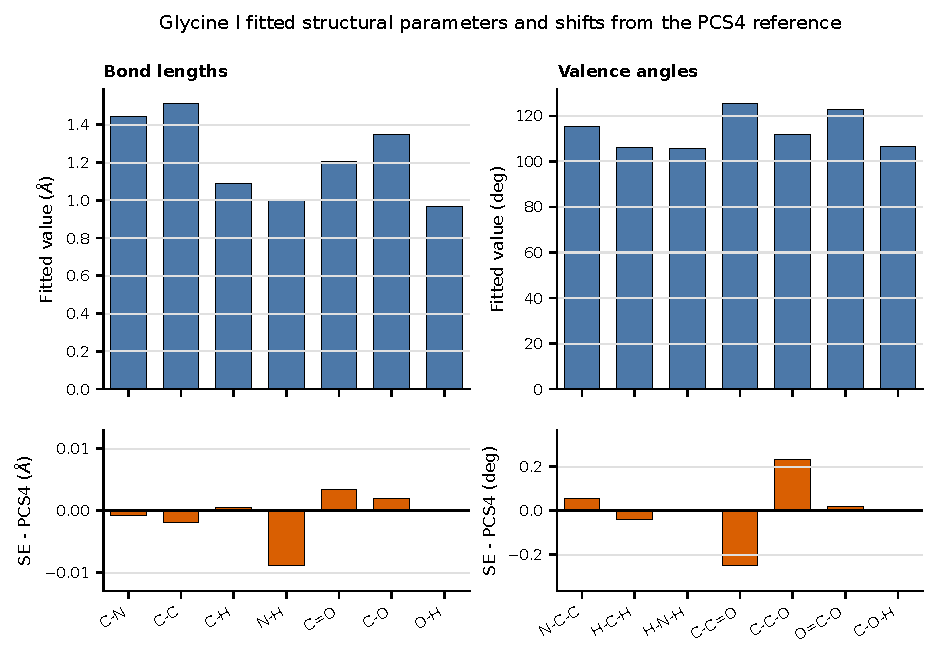
\includegraphics[width=0.94\linewidth]{figures/glycine_I_qc_fit_parameters.pdf}
\caption{Glycine I fitted structural parameters and shifts from the QC
reference geometry. The upper panels report final SE bond lengths and
valence angles; the lower panels report signed SE--QC differences on
expanded scales.}
\label{fig:glycine-I-qc-parameters}
\end{figure*}

The Gly-I structural comparison in
Figure~\ref{fig:glycine-I-qc-parameters} shows the scale of the
semiexperimental correction when the starting QC geometry already reproduces
the rotational data well. Since the reduced-dimensionality constraints are
generated from the QC reference structure, the small SE--QC differences
provide an a posteriori validation of the generated constraint
model, not merely a check that the starting geometry was good.

Detailed atom numbering, rotational constants, topological parameters,
Kraitchman diagnostics, reference-geometry comparisons, residuals, conditioning, and
covariance diagnostics are reported in the Supporting Information. The main text 
retains the information needed to
assess model formulation: rank, dimensionality, symmetry, constraint
projection, planar-component choice, residual scale, and minimum checks.

\subsection{Generated Reduced-Dimensionality Models}

Incomplete isotopic coverage can leave some structural directions unsupported.
The advisor therefore treats reduced dimensionality as part of the
model-generation step. It preserves the highest compatible symmetry, identifies
local coordinates that cannot be determined independently, and replaces them
by primitive-coordinate constraints, predicates, or parameter classes. 

\begin{table*}
\caption{Autonomous structural-model decisions made by the advisor in the
reduced-dimensionality benchmarks. ``Active variables'' are the
independent least-squares coordinates after symmetry selection and projection
of hard primitive-coordinate constraints.}
\label{tab:advisor-decisions}
\scriptsize
\setlength{\tabcolsep}{2.5pt}
\begin{tabular}{lllll}
\toprule
System & GIC space & Variables & Auto constraints & Classes \\
\midrule
Glycine I & 24 GICs; 15 $A'$ & 11 & 4 QC functional constraints & none \\
Glycine II & 24 GICs; C$_1$ & 19 & 5 QC functional constraints & coupled descriptors \\
Norcamphor & 48 GICs; C$_1$ & 18 & 30 hydrogen-frame constraints & constrained H frames \\
\bottomrule
\end{tabular}
\end{table*}

Table~\ref{tab:advisor-decisions} shows that the reduced models are generated
from isotope coverage and chemical equivalence rather than imported as a
manual parameter subset. In glycine I, glycine II, and norcamphor the available
substitutions do not support all hydrogen-related directions independently;
the advisor therefore converts the unsupported directions into explicit
primitive-coordinate relations derived from the reference structure.

\subsection{Glycine as an End-to-End Model-Generation Test}

The two glycine conformers test the same model-generation layer starting
from QC geometries when hydrogen-related directions are only partly supported. 

\begin{figure*}
\centering
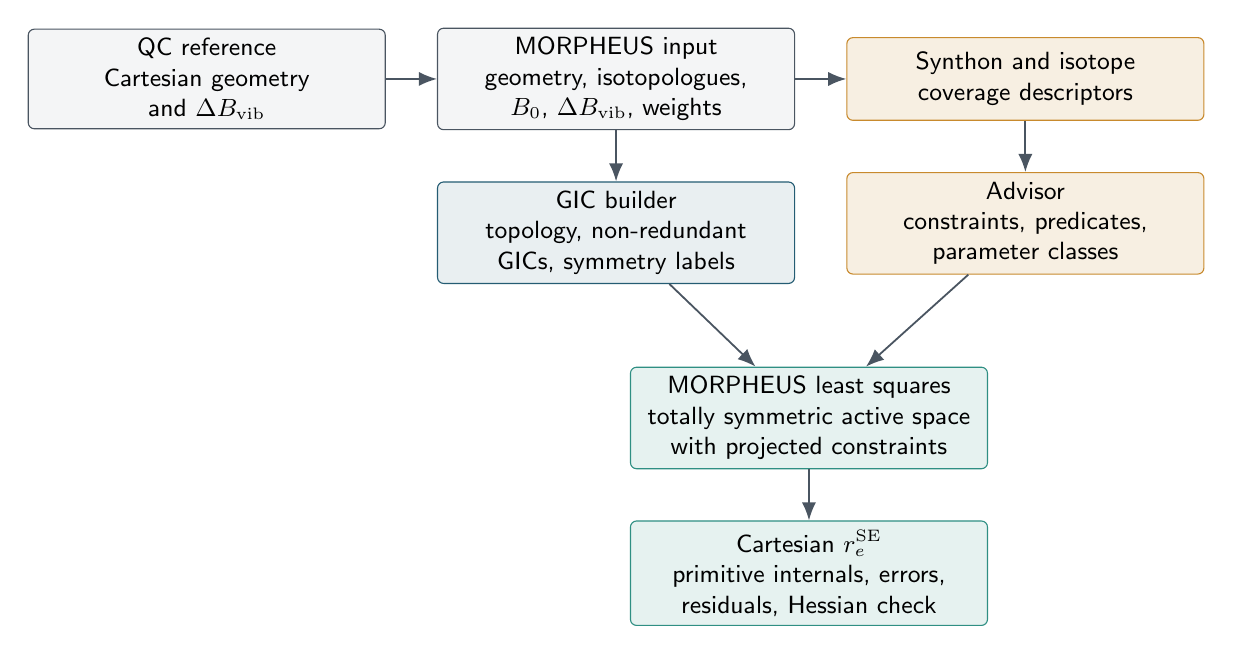
\begin{tikzpicture}[
  node distance=0.65cm,
  stepbox/.style={
    draw=FrameworkSlate,
    fill=FrameworkSlate!6,
    rounded corners=2.2pt,
    align=center,
    text width=4.3cm,
    minimum height=1.05cm,
    font=\small\sffamily
  },
  autobox/.style={stepbox, draw=FrameworkBlue, fill=FrameworkBlue!10},
  chemobox/.style={stepbox, draw=FrameworkGold, fill=FrameworkGold!14},
  fitbox/.style={stepbox, draw=FrameworkTeal, fill=FrameworkTeal!12},
  flowarrow/.style={-{Latex[length=2.3mm,width=1.8mm]}, line width=0.65pt, draw=FrameworkSlate}
]
\node[stepbox] (pcs) {QC reference\\Cartesian geometry\\and $\Delta B_\mathrm{vib}$};
\node[stepbox, right=0.65cm of pcs] (job) {MORPHEUS input\\geometry, isotopologues,\\$B_0$, $\Delta B_\mathrm{vib}$, weights};
\node[chemobox, right=0.65cm of job] (syn) {Synthon and isotope\\coverage descriptors};
\node[chemobox, below=0.65cm of syn] (adv) {Advisor\\constraints, predicates,\\parameter classes};
\node[autobox, below=0.65cm of job] (gic) {GIC builder\\topology, non-redundant\\GICs, symmetry labels};
\node[fitbox, below=1.05cm of gic, xshift=2.45cm] (fit) {MORPHEUS least squares\\totally symmetric active space\\with projected constraints};
\node[fitbox, below=0.65cm of fit] (out) {Cartesian $r_e^\mathrm{SE}$\\primitive internals, errors,\\residuals, Hessian check};
\draw[flowarrow] (pcs) -- (job);
\draw[flowarrow] (job) -- (syn);
\draw[flowarrow] (syn) -- (adv);
\draw[flowarrow] (job) -- (gic);
\draw[flowarrow] (gic) -- (fit);
\draw[flowarrow] (adv) -- (fit);
\draw[flowarrow] (fit) -- (out);
\end{tikzpicture}
\caption{End-to-end algorithmic glycine refinement starting from QC Cartesian reference 
geometries and vibrational corrections.
The workflow uses the common job/xyzin container, chemical descriptors, and isotope
coverage to generate the active coordinate and constraint model without manually 
selected fit variables.}
\label{fig:glycine-algorithmic-flow}
\end{figure*}

For glycine I, the parent, $^{13}$C(carboxyl), $^{13}$C(methylene), CD$_2$,
and $^{15}$N isotopologues are fitted using the rotational constants and
weights of Godfrey and Brown\cite{GodfreyBrown1995ShapeGlycine} and the
zero-point corrections of Kasalov{\'a} et al.\cite{Kasalova2007Glycine} The
QC reference already reproduces the 15 vibrationally corrected constants
with an RMS relative error of 0.0258\% and a maximum error of 0.0363\%. The
advisor detects the C$_s$ geometry and incomplete hydrogen information and
generates four constraints: O--H distance, C--O--H angle, H--N--H angle, and
NH$_2$ wag. Projection leaves 11 independent variables from 15 $A'$ GICs, and
the final fit gives a complete rotational RMS residual of 0.0269 MHz with a
positive optimized-space Hessian.

\input{generated/glycine_I_qc_rotational_comparison}

The Gly-I comparison is intentionally stringent: the refinement starts from an already
spectroscopically consistent QC structure rather than correcting a poor
starting point. Since the reduced-dimensionality constraints are generated
from the QC reference structure, the small SE--QC differences provide an
a posteriori validation of the generated constraint model. The
largest heavy-atom bond and valence-angle shifts relative to the final
semiexperimental structure are 0.0034~\AA\ and 0.25$^\circ$, respectively,
both within the scale expected for state-of-the-art QC structures and vibrational
corrections.\cite{PuzzariniStanton2023,Mendolicchio2025FastDvib}

Glycine II is the non-symmetric reduced-dimensionality case. The available
isotopologues do not determine a stable full structure, so the QC reference
is used to generate coupled primitive-coordinate constraints: C--H and N--H
differences, two methylene angular combinations, and an average H--N--C--C
torsion. These constraints are then projected onto the
24-dimensional C$_1$ GIC space.

\begin{table}[htbp]
\caption{Glycine II constraint-source comparison. Both calculations used GIC coordinates, moments of inertia as observables, and the same 10 corrected Gly-IIn rotational data sets. Rotational residuals are reported over the diagnostic $A$, $B$, and $C$ constants in MHz. The last column is the mean-square convention used for comparison with the published glycine refinement, not a second RMS value.}
\label{tab:glycine-constraint-comparison}
\begin{tabular}{lrrrr}
\toprule
Constraint target source & Rank & RMS & Max & $10^3\langle\Delta B^2\rangle$ \\
\midrule
Kasalov{\'a}-type values & 19 & 0.2344 & 0.8100 & 54.94 \\
QC-derived values & 19 & 0.2491 & 0.6707 & 62.06 \\
\bottomrule
\end{tabular}
\end{table}

Table~\ref{tab:glycine-constraint-comparison} shows that QC-derived targets
produce the same rank and essentially the same residual scale as the published
Kasalov{\'a}-type constraints. The final QC-constrained refinement has 19
effective variables, a condition number of $1.05\times10^4$, and a complete
rotational RMS residual of 0.2491 MHz. The largest uncertainties remain in the
amino-hydrogen frame, as expected from the substitution pattern.

\subsection{Testosterone: Large-Molecule Scale Demonstration}

The validation benchmarks above were selected because they represent available
experimental gold standards while spanning acyclic, cyclic, fused, bridged,
planar, homologous, and reduced-dimensionality cases. The model-generation
layer is not limited to these sizes. As a scale check, the framework was
also applied to testosterone, using the published experimental ground-state
rotational constants and vibrational corrections for the observed
T1-H2$^{-}$-gp conformer.\cite{Uribe2024SteroidHormones} This is a useful large
molecule test because this level of treatment is rarely available for systems
of this size: an accurate QC equilibrium geometry, accelerated
$\Delta B_\mathrm{vib}$ corrections, and algorithmic model generation are
combined in one black-box protocol.

The unrefined QC+$\Delta B_\mathrm{vib}$ residuals with respect to the corrected
experimental constants are $4.638$, $0.674$, and $0.563$ MHz for $A$, $B$, and
$C$, respectively. After a 141-dimensional non-redundant space is built, the
class layer applies a single topology-derived C--C skeletal stretch class.
Operationally, non-skeletal stretch combinations and the angular, torsional,
and out-of-plane families are held fixed for this parent-only diagnostic, while
the retained C--C stretch block is replaced by one shared variable after rank
reduction. The resulting refinement improves the residuals to $-0.027$,
$0.633$, and $0.291$ MHz, reducing the RMS rotational residual from 2.73 to
0.40 MHz. This test is deliberately not presented as an isotope-rich structural
validation: it demonstrates that a large-molecule QC geometry, vibrational
corrections, non-redundant coordinate generation, and class-constrained
refinement can be chained for a 49-atom fused-ring molecule, where sufficiently
rich isotopic substitution data are not presently available for a full
validation of the fit engine.

\begin{figure}
\centering
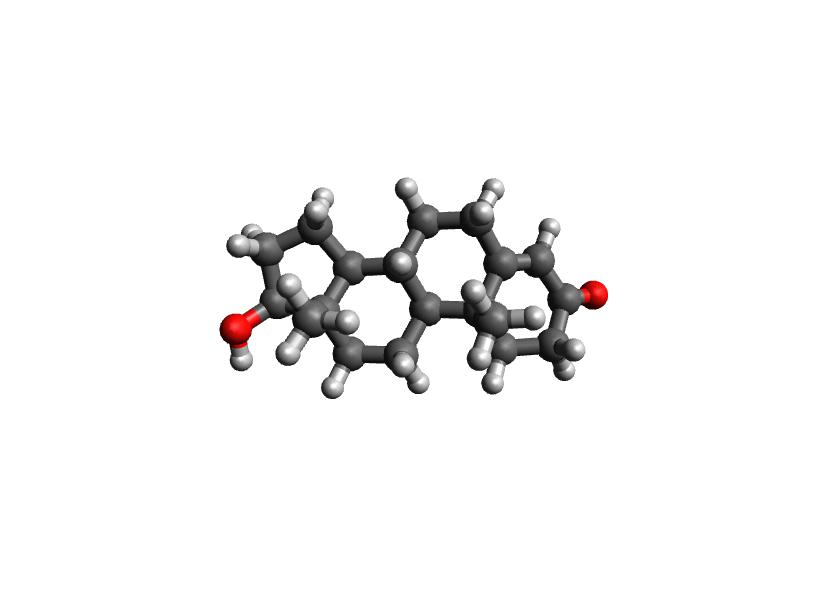
\includegraphics[width=0.72\linewidth]{figures/testosterone_qc.jpg}
\caption{Testosterone T1-H2$^{-}$-gp large-molecule scale demonstration.}
\label{fig:testosterone-scale-check}
\end{figure}

\begin{table}[htbp]
\caption{Testosterone T1-H2$^{-}$-gp scale check. Residuals are relative to
the corrected experimental equilibrium constants derived from the published
$B_0$ and $\Delta B_\mathrm{vib}$ values.}
\label{tab:testosterone-scale-check}
\begin{tabular}{lrrrr}
\toprule
Model & Variables & $\Delta A$ & $\Delta B$ & $\Delta C$ \\
\midrule
QC+$\Delta B_\mathrm{vib}$ & 0 & 4.638 & 0.674 & 0.563 \\
Class-constrained fit & 1 & -0.027 & 0.633 & 0.291 \\
\bottomrule
\end{tabular}
\end{table}

\section{Conclusions}

The central contribution of this work is to move semiexperimental model formulation into a
single auditable algorithm. Existing refinement methods generally assume that
the coordinate model has already been supplied; here topology perception,
symmetry assignment, homogeneous rank pruning, constraint projection,
least-squares solution, and covariance propagation are part of one calculation
rather than separate user decisions.

The benchmarks show that the resulting models remain topology-derived,
symmetry-consistent, rank-consistent, and non-redundant for acyclic, cyclic,
planar, fused, bridged, homologous anhydride, glycine, and large fused-ring
cases. The program selects the active symmetry space, removes redundant
coordinates, chooses the independent moment components for planar molecules,
generates constraints when isotopic coverage is incomplete, and propagates
covariance to the reported structural parameters. Where both active coordinate
models are applicable, GIC and symmetry-Cartesian refinements give the same
effective dimensions and rotational residuals.

Electronic-structure information is used only where the experiment does not
fully determine the structure. For Gly-I the QC reference already lies within
the practical rotational-accuracy window, so the fit provides a
statistically consistent semiexperimental correction and uncertainty estimate.
For Gly-II and norcamphor, the advisor converts reference information and
isotope coverage into explicit reduced-dimensionality constraints. The
reference therefore supplies constraints for unsupported directions, while the
spectroscopic data determine all supported directions.

This is not simply a convenient input generator. The final outputs remain
ordinary chemical objects: Cartesian structures, bond lengths, valence angles,
dihedrals, ring descriptors, propagated uncertainties, residuals, and
diagnostics. What changes is that the path from topology and data to those
objects is explicit, reproducible, and rank-audited, even for molecular graphs
in which manual coordinate formulation is often the limiting step.

The testosterone scale check extends this logic to the current upper end of
practical rotational-spectroscopic modeling. It does not claim a complete
semiexperimental structure from a parent-only data set; instead, it shows that
an accurate large-molecule QC geometry, accelerated $\Delta B_\mathrm{vib}$
corrections, algorithmic non-redundant GIC generation, and class-constrained
refinement can be chained for a 49-atom fused-ring molecule in a
reproducible black-box calculation. This closes the loop from accurate
large-molecule QC structures to algorithmically generated spectroscopic
refinement models.
The essential shift is from expert-dependent model formulation to reproducible
algorithmic model generation.

\section*{Supporting Information Available}

Atom-numbered structures for the benchmark and companion systems; complete
rotational-constant comparisons for glycine I, glycine II, cyclopentadiene,
nitrobenzene, and azulene; Kraitchman, reference-fit, and planar-component
diagnostics; additional diagnostic tables for glycolaldehyde and norcamphor;
final Cartesian coordinates, propagated topological parameters, residuals, and
archived \texttt{MORPHEUS} output files.


\bibliographystyle{aipnum4-2}
\bibliography{references}

\end{document}
